\documentclass{acmsmall}

\usepackage[ruled]{algorithm2e}
\usepackage{graphicx}
\graphicspath { {images/} }
\renewcommand{\algorithmcfname}{ALGORITHM}
\SetAlFnt{\small}
\SetAlCapFnt{\small}
\SetAlCapNameFnt{\small}
\SetAlCapHSkip{0pt}
\IncMargin{-\parindent}

\setcopyright{rightsretained}

% Document Start
\begin{document}

% Page heads
\markboth{Roger Ogden and Brik Royster}{Arbitrary Code Execution}

% Title portion
\title{Arbitrary Code Execution}
\author{ROGER OGDEN AND BRIK ROYSTER}

\begin{abstract}
% TODO: this is not an abstract
suh dude
\end{abstract}

%
% The code below should be generated by the tool at
% http://dl.acm.org/ccs.cfm
% Please copy and paste the code instead of the example below. 
%
\begin{CCSXML}
<ccs2012>
<concept>
<concept_id>10002978.10003022.10003023</concept_id>
<concept_desc>Security and privacy~Software security engineering</concept_desc>
<concept_significance>300</concept_significance>
</concept>
</ccs2012>
\end{CCSXML}

\ccsdesc[300]{Security and privacy~Software security engineering}

%
% End generated code
%

\terms{Security}

\keywords{Arbitrary code execution, code injection}

\acmformat{Roger Ogden and Brik Royster, 2016. Arbitrary Code Execution}

\begin{bottomstuff}
Authors' addresses: Roger Ogden and Brik Royster,
College of Engineering, Computer Science Department
Boise State University
\end{bottomstuff}

\maketitle

\section{Introduction}

Arbitrary code execution is a type of injection exploit in software, relating to many well-known exploit concepts, including Shellshock, email injection, and cross-site scripting. Arbitrary code execution refers to the process by which one or more processes running in a program are compromised, allowing code to be ran that wasn’t intended to be. Traditionally, it’s assumed the goal of arbitrary code execution is a malicious one, such as the theft of information or corruption of data, but that’s not always the case. There are instances where arbitrary code execution are used for research and entertainment purposes, such as finding ways to beat video games faster than would be possible under normal conditions, or to generate an entirely new experience using the game’s assets. In any case, arbitrary code execution is an evergreen topic because of the impact is has on the software industry, with security in software being paramount. In this paper, we will discuss several aspects of arbitrary code execution, citing and explaining examples along the way.

\section{A Brief History of Arbitrary Code Execution}

Arbitrary code execution has been around since assembly programming was commonplace. At its simplest form, arbitrary code execution is a software bug, not the result of a brute-force attack on a resource, such as trying millions of passwords on a particular website to steal the information of a particular user. That is, arbitrary code execution is, theoretically, preventable.

Because arbitrary code execution has been a software engineering issue for so long, it comes in many forms. Some of the most famous examples of arbitrary code execution were a result of bugs in standard C programming libraries, with \texttt{strcpy} being the most famous. Moreover, the \texttt{fingerd} daemon in Linux was known to have a vulnerability that allowed buffer overflow, and consequently, any user to execute local binaries.

Today, the web is perhaps the most common place for arbitrary code execution to occur. In 2012, the Foxypress Wordpress plugin was found to have an exploit that could allow arbitrary code execution. One of the plugin’s source code files, \texttt{uploadify}, was responsible for allowing users to upload remote files to their Wordpress servers. When the exploit was found, it allowed for remote files to execute malicious PHP code on the user’s Wordpress server. Potential outcomes of this bug include website vandalism, database corruption, and stealing of credit card (or any other) information. It was found that versions 0.4.1.1 - 0.4.2.1 were vulnerable (1). The source code containing the exploit can be seen in Figure 1.

Furthermore, In June 2016, it was found that Google Chrome’s PDF viewer had the potential for arbitrary code execution. In CVE-2016-1681, found by Aleksandar Nikolic, it was discovered that if a PDF has an embedded \texttt{jpeg2000} image could trigger a heap buffer overflow. The simple fix, according to Nikolic, was to change an \texttt{assert} statement to an \texttt{if} statement in the call to a  OpenJPEG library function that Google used in their PDF viewer. (4)

Lastly, Apple discovered a vulnerability in \texttt{configd}, a DNS networking daemon that is included on devices running iOS, their mobile operating system. A heap based buffer overflow issue existed in the DNS client library. A malicious application with the ability to spoof responses from the local \texttt{configd} service may have been able to cause arbitrary code execution in DNS clients. This bug was reported by PanguTeam, a team of hackers responsible for many versions of the programs that allowed users to “jailbreak” their iOS devices. (5)

\section{How Arbitrary Code Execution Works}

The possibility of all arbitrary code execution is reliant on the ability to obtain access to the instruction pointer for any particular program. The instruction pointer is a processor register that points to where the current program is executing in memory. Therefore, wherever the instruction pointer is, is what’s being executed at the current time slot for that particular program. Access to the instruction pointer allows for any user to manipulate where the instruction pointer is pointing, in turn allowing for arbitrary code execution. 

In \ref{fig:ip}, the instruction pointer sits between \textbf{L. Address} and \textbf{H. Address}, the address space for the currently executing program. During the instruction fetch stage of the pipelined CPU process, the instruction pointer takes the instruction at that address, and loads it into the instruction register to be used for decoding and execution. The instruction pointer then increments by an amount that varies depending on what type of instruction was fetched. For example, if the instruction was add, the instruction pointer might only increment by one. However, if the instruction was a jump command, the instruction pointer might jump further down the address space, as is evident in figure \ref{fig:ip}. Therefore, control over the instruction pointer is paramount for arbitrary code execution to occur. \cite{instruction_pointer_1999}

\begin{figure}
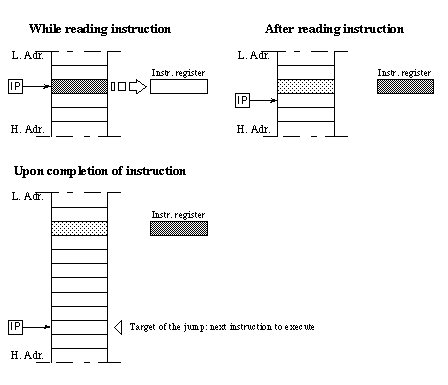
\includegraphics[width=\linewidth]{ip.png}
\caption{The process by which the instruction pointer moves.}
\label{fig:ip}
\end{figure}

\subsection{Buffer Overflow}

The most common way to obtain access to the instruction pointer is through buffer overflow. Buffer overflow is a simple concept made possible by flaws in programs that typically run with administrator privileges. Essentially, buffer overflow occurs when the input to a program or method in a program is larger than the developer of the program expected. As a result, the method has a way of overwriting the amount of stack memory that was allocating to it, putting the program in an unknown state. When the stack memory is overwritten, the program no longer has the capability of returning to the address that called the method. As a result, the tail end of the overwritten stack could have code that points to a different address, thus compromising the instruction pointer.

The most famous example of this is the use of \texttt{strcpy} in the C Standard Library. The implementation of \texttt{strcpy} is to copy each character until it finds a \texttt{0} in the source string, which is used to denote the end of the string. This function easily allows users to overwrite the stack memory, as referenced in figure \ref{fig:strcpy}. \cite{buffer_overflow_attack_2004}

Figure \ref{fig:shellcode} explains how to take advantage of a compromised instruction pointer. The character array called \texttt{shellcode} is filled with pre-written machine code that will open a shell on the compromised system. In the main method, by manipulating the value of ret initially to be pointing to the return address of main, and then manipulating that return address to be where the contents of \texttt{shellcode} are stored, a user can execute the contents of \texttt{shellcode}.

The process by which the machine code for \texttt{shellcode} was generated can be used for any code a user would want to arbitrarily execute. The origins of \texttt{shellcode} is a simple C program:

\begin{lstlisting}[language=C]
#include <stdio.h>

void main() {
   char *name[2];

   name[0] = "/bin/sh";
   name[1] = NULL;
   execve(name[0], name, NULL);
}
\end{lstlisting}

In order to determine the assembly code that is generated from the C program, a user could use \texttt{gdb}, a popular open-source debugger for C and assembly programs. After careful examination of the \texttt{gdb} output, it's possible to determine the assembly code that would be needed to perform a system call that executes the contents of the \texttt{shellcode} program. After the assembly instructions have been determined, generating the machine code is only a matter of compiling the assembly. Following that, a user could compile their code with \texttt{gcc} such that their program is placed in the global data segment, making it both readable and writable by the operating system. A user could then have code that is ready to be injected into a compromised process for arbitrary code execution.

\newpage
\vfill

\begin{figure}
\begin{lstlisting}
#include <string.h>
#include <stdio.h> 

void foo(const char* input)
{
    char buf[10];

    printf("My stack looks like:\n%p\n%p\n%p\n%p\n%p\n% p\n\n");

    strcpy(buf, input);
    printf("%s\n", buf);

    printf("Now the stack looks like:\n%p\n%p\n%p\n%p\n%p\n%p\n\n");
}

void bar(void)
{
    printf("Augh! I've been hacked!\n");
}

int main(int argc, char* argv[])
{
    //Blatant cheating to make life easier on myself
    printf("Address of foo = %p\n", foo);
    printf("Address of bar = %p\n", bar);
    if (argc != 2) 
    {
        printf("Please supply a string as an argument!\n");
        return -1;
    } 
    foo(argv[1]);
    return 0;
}
\end{lstlisting}
\caption{An example of using buffer overflow to overwrite stack memory.}
\label{fig:strcpy}
\end{figure}

\begin{figure}
\begin{lstlisting}
char shellcode[] =
  "\xeb\x2a\x5e\x89\x76\x08\xc6\x46\x07\x00\xc7\x46\x0c\x00\x00\x00"
  "\x00\xb8\x0b\x00\x00\x00\x89\xf3\x8d\x4e\x08\x8d\x56\x0c\xcd\x80"
  "\xb8\x01\x00\x00\x00\xbb\x00\x00\x00\x00\xcd\x80\xe8\xd1\xff\xff"
  "\xff\x2f\x62\x69\x6e\x2f\x73\x68\x00\x89\xec\x5d\xc3";


void main() {
  int *ret;


  ret = (int *)&ret + 2;
  (*ret) = (int)shellcode;
}
\end{lstlisting}
\caption{The contents of \texttt{shellcode} are executed when the return address of the main method is manipulated.}
\label{fig:shellcode}
\end{figure}

\vfill
\clearpage


\section{How Arbitrary Code Execution Can Be Prevented}

Because of the potentially catastrophic situations that can arise from arbitrary code execution exploits, several methods for preventing it have been implemented. Most end-all solutions take place in the C compiler (such as gcc); solutions for other languages like Bash tend to more specific to individual exploits that have occurred.

One low-level solution for preventing arbitrary code execution is the inclusion of a no-execute (NX or XD depending on the processor) bit on the CPU. In essence, this method marks certain parts of memory executable (such as the .text segment in a program), while leaving other parts of memory marked as non-executable (such as the .data segment in the program). Then, before executing any instructions, the CPU checks this no-execute bit to see if the memory it is executing from should be executed or not. If the instruction pointer ever moves to a place in memory that is not marked as executable, the program faults and exits. The inclusion and usage of a no-execute bit has been present in Windows since Windows XP SP2 (7). This method is very good in preventing code being executed from portions of memory that are controlled by the user (such as strings built from user input), but it does not stop every exploit. For instance, the Dirty COW exploit on Linux that arose recently took advantage of rewriting the .text segment, so even a no-execute bit couldn’t have prevented arbitrary code from being executed.

Another solution that is in-use today by gcc is the inclusion of a stack canary during execution. The idea behind this is that most (not all) arbitrary code execution exploits take advantage of manipulating the call stack to return execution to a new place in memory and ultimately execute code that was not intended to be executed. In an attempt to prevent this, a small random integer is placed just before the call stack in memory. Since the most common way to overwrite the stack is to overflow memory writing from normal memory into the stack, any code trying to write its way into the call stack will have to overwrite the stack canary (8). This canary value is checked often, and if it is ever not equal to the original random value it was assigned, then the stack might have been manipulated and the program faults. Of course, like the no-execute bit, this solution is not full proof. In fact, the same exploit that bypasses an no-execute bit (Dirty COW) could bypass a stack canary just as easily.

Basic prevention of arbitrary code execution can stop many exploits from ever occurring, but a program is almost never truly safe. Even if a program is written and compiled with extreme care, bugs can still be exploited in the compiler or operating system. Developers should always be aware of the third-party libraries they are using in their programs and pay attention to any potential exploits that can arise from them. They should also make sure to always use the safe copying functions in C (such as strncpy instead of strcpy). Finally, they should be proactive in fixing any bugs that show signs of allowing arbitrary code execution to exist. Even if fixes are implemented and updates are launched the day an exploit is discovered, machines that aren’t up to date can still be compromised and huge problems can still occur.

\section{Case Study: Arbitrary Code Execution in \textit{Super Mario World}}

One great example of arbitrary code execution not being used for evil can be found in speedruns and tool-assisted play of various classic video games. In essence, a speedrun is trying to beat a video game as quickly as possible; using glitches and other unintended tricks are generally allowed and encouraged.

In several classic video games (such as \textit{Super Mario World} for the SNES), glitches exist that allow arbitrary code execution to be possible. The methods for performing and taking advantages of these glitches varies from game to game, but they tend to exist more often in older video games due to the smaller memory capacities of the retro consoles and the somewhat questionable techniques game developers used to overcome the constraints. Most cases of arbitrary code execution in video games simply result in jumping to a certain instruction in game code (e.g. the final credits) to skip large portions of the game. However, some games can be coerced into a state where inputs from the controller directly map to assembly instructions being executed by the console. This is known as total control.

To showcase an example of how powerful arbitrary code execution can be for speedruns, we will examine the methods used to beat \textit{Super Mario World} in under two minutes by a human player \cite{dotsarecool_2015}.

\subsection{Constructing the Arbitrary Code}

The basis of this glitch is that the player is able to use an array in the game's memory that normally stores the positions of various sprites on screen as a set of instructions to be executed that will ultimately jump game execution to the final credits. This array that stores sprite locations has a maximum size of 12 elements, and whenever a new sprite is rendered on screen, it tries to place it in the highest available index in the array. Because of this, the lower elements in the array are only ever accessed or changed when there is a large number of sprites on the screen, which makes it easy to keep them at the values the player wants. In the pursuit of efficiency, sprite positions are only ever updated when the sprite moves, and are not cleared when a sprite leaves the screen for any reason. This means sprites can be placed in a very specific location, despawned using in-game mechanics, then as long as a new sprite is not ever placed in that sprite slot, the memory still has the correct values.

Conveniently, at the very beginning of the first level, a large number of enemies appear on screen and fill up the entire sprite array (this was probably placed there by the game designers to showcase how many enemies the game can handle at once on the new hardware the game was released on). The player can very carefully despawn these enemies (by eating them and spitting them out with Yoshi) at very specific locations to write some machine code to be executed later.

\begin{figure}
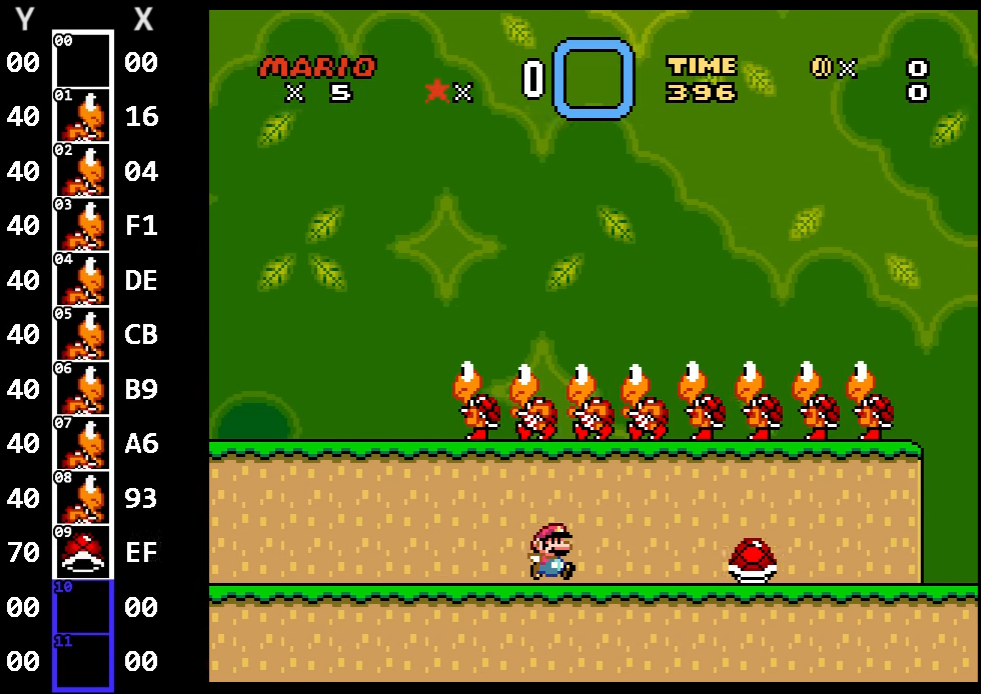
\includegraphics[width=\linewidth]{smw1.png}
\caption{The large number of enemies at the beginning of the game. To the left is a visualization of the sprite array, showing the low-bytes of Y and X positions of each sprite. These values are what is turned into code to be executed later on. \cite{dotsarecool_2015}}
\end{figure}

Once the code has been written using sprites, the player can then execute a very complicated glitch that allows program execution to jump to the sprite array's location in memory. The glitch involves attempting to eat a normal item with Yoshi at a specific spot in the level at the exact same time Mario jumps off of Yoshi and moves the screen to the right. When the screen moves enough to the right, it spawns another enemy in the level. However, since the item being eaten has already been despawned, the enemy spawns in the same sprite slot it was just occupying. Since Yoshi is still in the process of eating whatever item was in that sprite slot, it is able to eat the enemy that is not normally able to be eaten.

\subsection{Executing the "Shell" Code}

When Yoshi eats objects in \textit{Super Mario World}, the game looks at a large array of memory locations mapped to each eatable object (this is called a jump table). However, since the enemy being eaten isn't supposed to be in this array in the first place, the index the game tries to access in the jump table is way out of bounds and the game attempts to jump execution to an essentially random place in memory. This location isn't actually random, but it's the result of turning some other memory in the game near the jump table into an address and jumping to it. The other memory it reads happens to be the Y-position of the last particle objects drawn on the screen, which the player was also able to manipulate.

\subsubsection{Machine Code Explanation}

After performing this jump instruction from eating the invalid memory, the game is able to work its way into the sprite array and start executing code from there. The code written in the sprite array is the following:

      \begin{lstlisting}
      LDA #$1C   // A9 1C
      STA ($75)  // 92 75
      JMP $FF46  // 4C 46 FF
      \end{lstlisting}

\texttt{LDA \#\$1C}: Load the value \texttt{1C} into the accumulator. \texttt{1C} corresponds to the game mode that tells the game to fade out and start playing the credits.

\texttt{STA (\$75)}: Store the accumulator value indirectly at the address \texttt{\$75}. The address \texttt{\$75} is \texttt{01} if Mario is swimming, and \texttt{00} otherwise. Address \texttt{\$76} is \texttt{01} if Mario is facing right and \texttt{00} if Mario is facing left. As long as Mario is facing right and not swimming at the time the glitch is performed, the value \texttt{1C} will be stored at address \texttt{01 00}, which is where the current game mode is stored in memory.

\texttt{JMP \$FF46}: Normally, eating an invalid enemy would crash the game, so execution is jumped to a subroutine intended to draw a specific boss on the screen. This subroutine causes some interesting graphical glitches, but doesn't crash the game. Once the subroutine returns, the game realizes its state is the credits and launches the proper routine to to start playing them, thus beating \textit{Super Mario World}.

\begin{figure}
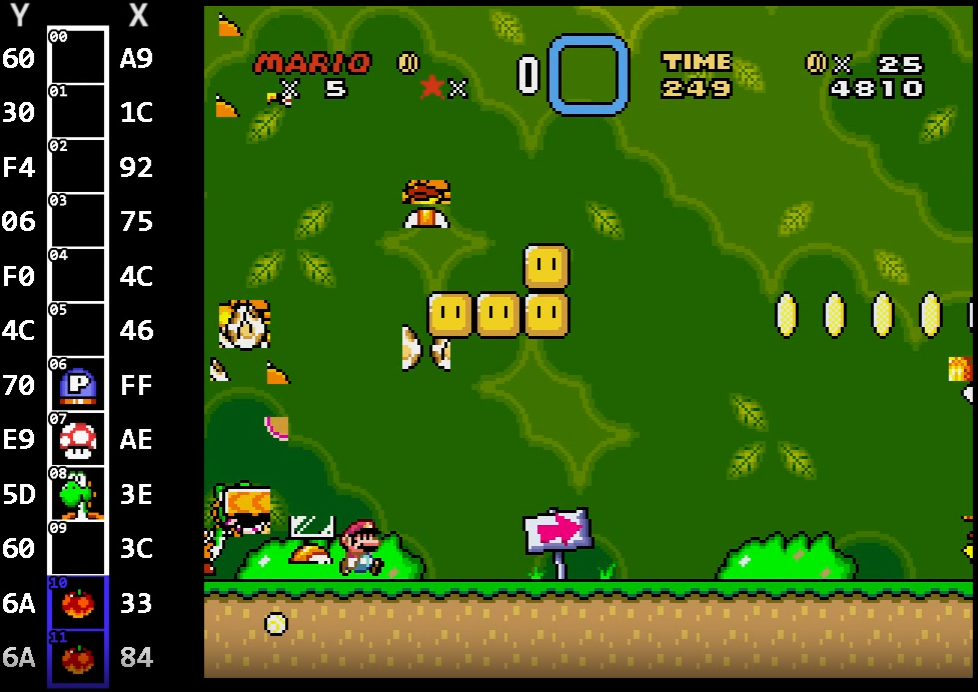
\includegraphics[width=\linewidth]{smw2.png}
\caption{The graphical glitches that occur when jumping to the boss-drawing subroutine. On the left, the same sprite array visualization shows the now complete machine code written via the X-positions of the first 7 sprite slots. \cite{dotsarecool_2015}}
\end{figure}


% Bibliography
\nocite{*}
\bibliographystyle{ACM-Reference-Format-Journals}
\bibliography{paper-bib}

\end{document}
